\subsection{Blockchain Structure}
A blockchain is a distributed, append-only ledger that maintains a continuously growing list of records, called blocks, securely linked together using cryptography. Each block contains a cryptographic hash of the previous block, a timestamp, and transaction data \cite{nakamoto2008bitcoin}. This structure ensures data integrity and immutability. 

A foundational component of this structure is the Merkle tree, which allows for efficient and secure verification of large data structures. By hashing pairs of nodes recursively until a single root hash is produced, a Merkle tree condenses vast amounts of transaction data into a single, succinct cryptographic commitment. This mechanism is extensively used in both Layer-1 blockchains (e.g., to summarize block transactions) and Layer-2 rollups (e.g., Sparse Merkle Trees to track state updates).
\begin{figure}[H]
    \centering
    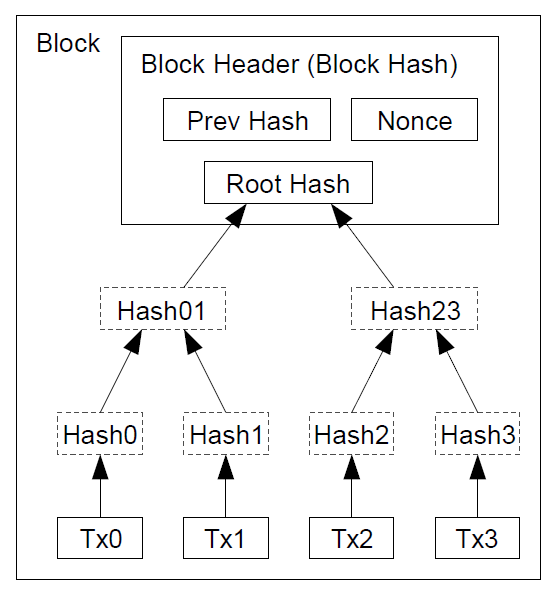
\includegraphics[width=0.90\textwidth]{figures/chapter1/merkle_tree.png}
    \caption{Merkle Tree structure representing transactions.}
    \label{fig:merkle_tree}
\end{figure}

As shown in Figure~\ref{fig:merkle_tree}, a Merkle tree allows for efficient and secure verification of large data structures.
